% !TEX encoding = UTF-8 Unicode
%!TEX root = ../Main/thesis.tex
% !TEX spellcheck = en-US
%%=========================================
\documentclass[../Main/thesis.tex]{subfiles}
\begin{document}
\chapter[One class SVM coupled with wavelet transform for bearing health monitoring]{One class SVM coupled with wavelet transform for bearing health monitoring}
\label{sec:waveletandsvm}
In this chapter we introduce yet a another method for bearing fault detection. In Chapter \ref{sec:chapter2} We showed how the fast Fourier transform is applied to bearing fault diagnosis. Although popular in the industry for bearing fault analysis and detection, the fast Fourier transform method is not without limitations. As in any scientific methods, the limitations are grounded in the mathematical assumptions upon which the method is derived. As pointed previously, two such assumption are linearity, and stationarity. Furthermore, for bearing fault analysis, the fast Fourier method relies on the rotational speed of the motor on which the bearings are mounted. In addition, the forcing frequencies are derived from the physical properties of the bearing. Thus, the fast Fourier transform method for bearing fault detection can be seen as a physics base data driven method.
\justify
In this chapter, a purely data driven method is presented. It consists of applying wavelet transform for feature generation, a robust statistical estimator to quantify a bearing health, and a support vector machine (SVM) for anomaly detection. Before giving a detail account of the method, let clarify some semantics and outline the benefits of this method. A feature in the context of this chapter, is a component of a signal. As pointed out earlier, a signal can have multiple components, which can be extracted for example by applying Fourier series or Fourier transform. In this case a feature or component of the original signal is a trigonometric function. A support vector machine (SVM) is a linear classification algorithm for pattern identification that uses margins to separate data into different groups [vapnik1995].
\justify
The method presented in this chapter solely relies on the data to detect any fault. it does not require bearing physical properties, and can be applies to any nonlinear and non-stationary data generated process. In the rest of this chapter we will refer to a generic bearing fault as an anomaly. As defined in [chandola2009], \say{Anomalies are patterns in data that do not conform to a well defined notion of normal behavior}. In section \ref{sec:svm} a detailed account of support vector machine algorithm is lade out, followed by wavelet transform in section \ref{sec:wavelet}. Finally, section \ref{sec:sectionresult} presents a one class SVM coupled with wavelet transform for bearing anomaly detection.

%%%%%%%%%%%%%%%%%%%%%%%%%%%%%%%%%%%%%%%%%%%%%%%%%%%%%%%%%%%%%%%%%%%%%%%%%%%%%%%%%%%%%%%%%%%%%%%%%%%
%%%%%%%%%%%%%%%%%%%%%%%%%%%%%%%%%%%%%%%%%%%%%%%%%%%%%%%%%%%%%%%%%%%%%%%%%%%%%%%%%%%%%%%%%%%%%%%%%%%
\section{Support vector machine (SVM)}
\label{sec:svm}
The Support vector machine algorithm was originally derived by [vopnikk1995] as a two-groups, classification algorithm. It solves the problem of classifying an input vector into two groups. In the context of bearing fault detection: healthy versus unhealthy bearing would be the two groups. It was originally introduced as support-vector Networks, but is now popularly refer to as support vector machine. The bulk of the SVM rests on the following idea: Use a nonlinear kernel to map the input data into a high dimensional feature space, where a linear decision function is used to classify data into two groups [vopmik1995].
\justify
A non linear kernel is just a nonlinear function and a decision function also called a discriminator function is a curve that separates the two groups. The classification is based on optimizing a margin separating the two groups. 
\begin{figure}[H] %  figure placement: here, top, bottom, or page
   \centering
   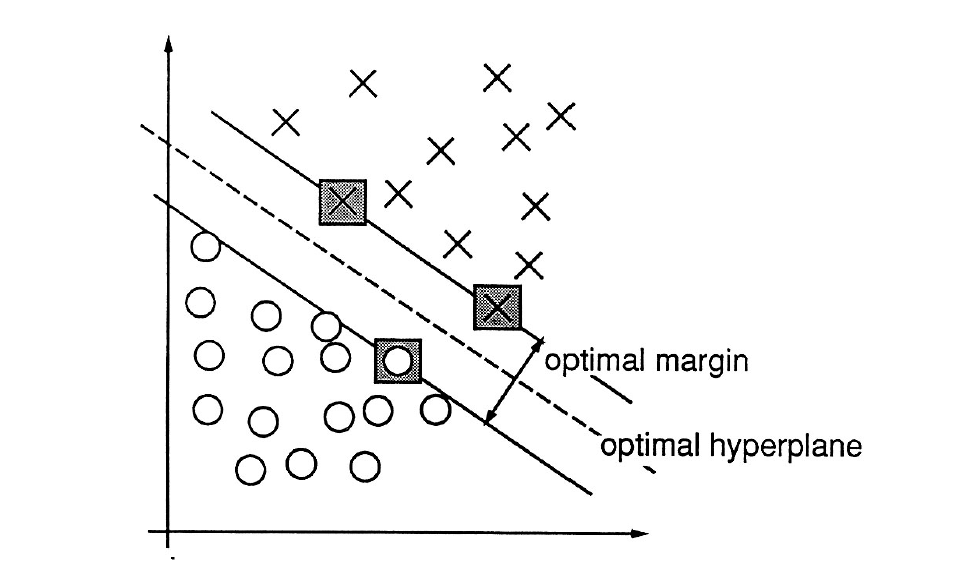
\includegraphics[width=5in]{../fig/svm2d.png} 
   \caption{Illustration of two classes classification from [vapnik1995]}
   \label{fig:svm2d}
\end{figure}
\justify
Figure \ref{fig:svm2d} shows a two groups classification problem. Two set of points marked by circle and cross are separated by the optimum curve or hyperplane (here the solid dash line). The margin is the distance or gap between solid dark lines. Here the two classes are linearly separable, meaning that a linear function can be used to separate the two classes. Support vectors are points that lies on the margins (points in grey square lying on the dark lines) and defines the margin of largest separation between the two classes [vapnik1995].
\justify
The SVM can be formulated as a convex quadratic optimization problem. In this setting, the objective function is convex and quadratic, and the inequality constraint is convex. Henceforth, from the duality principal of the mathematical optimization theory, there exist two formulations of the SVM: A primal formulation and an equivalent dual formulation. For convex optimization problem, we always nearlly have strong duality, that is the optimum solution of the primal problem is equal to the optimum solution of the dual problem.

\justify
The formulation of the SVM problem goes like this: Find the optimum linear curve (the dash line in Figure \ref{fig:svm2d}), that separates  two groups of points (circle points and cross points in Figure \ref{fig:svm2d}), from the nearest points of each class (the support vectors which are points in the in grey square in Figure \ref{fig:svm2d}).
\justify
Let $\bm{X}_{i} \in \mathbb{R}^{d}$  be an input vector, $\bm{W}\in \mathbb{R}^{d}$ a vector of parameters and $b\in \mathbb{R}$, where $d$ is an integer. Let $y_{i}\in \{-1,1\}$. Any vector $\bm{X}_{i}$ can be classify as 
\begin{equation}\label{eq:svmformulation}
y_{i} =
  \begin{cases}
                                   -1 & \text{if $\bm{W}^{T}\bm{X}_{i} + b < 0$} \\
                                   1 & \text{if $\bm{W}^{T}\bm{X}_{i} + b > 0$},
  \end{cases}
\end{equation}
where the equation of the separating hyperplane is given by 
\begin{equation}\label{eq:svmformulation01}
\bm{W}^{T}\bm{X}_{i} + b = 0.
\end{equation}
The problem specified by equation (\ref{eq:svmformulation}, \ref{eq:svmformulation01}) can be formulated as the following convex quadratic optimization problem:
\begin{equation}\label{eq:svmformulation1}
\min_{\bm{W},b}\frac{1}{2}||  \bm{W}||^{2}
\end{equation}
subjected to 
\begin{equation}\label{eq:svmformulation2}
y_{i}\left( \bm{W}^{T}\bm{X}_{i} + b \right) \geq 0, \quad i = 1,\cdots,n.
\end{equation}
Equations (\ref{eq:svmformulation1}, \ref{eq:svmformulation2}) is called the primal formulation of the SVM. An equivalent dual formulation called the Lagrangian dual formulation is defined as followed:
Let 
\begin{equation}\label{eq:svmprime1}
L(\bm{W}, b, \theta) = \frac{1}{2}||  \bm{W}||^{2} -\sum_{i}^{n}\theta_{i}\left(y_{i}\left( \bm{W}^{T}\bm{X}_{i} + b \right) -1  \right)
\end{equation}
be the Lagrangian derived from the primal SVM formulation, where $\theta_{i} \in \mathbb{R}^{d}$, and $\bm{W}^{T}$ denotes the transpose of the vector $\bm{W}$. Taking the partial derivative of the Lagrangian with respect to $\bm{W}$ and $b$ we obtain  
\begin{equation}\label{eq:dual1}
\begin{split}
\frac{\partial L(\bm{W}, b, \theta)}{\partial \bm{W}} &= \bm{W}-\sum_{i=1}^{n}\theta_{i}y_{i}\bm{X}_{i} = 0, \quad \Rightarrow \bm{W} = \sum_{i=1}^{n}\theta_{i}y_{i}\bm{X}_{i}\\
\frac{\partial L(\bm{W}, b, \theta)}{\partial b} &= \sum_{i=1}^{n}\theta_{i}y_{i} = 0.
\end{split}
\end{equation}
Substituting $\bm{W}$ back to the primal formulation (\ref{eq:svmformulation1}, \ref{eq:svmformulation2}) , with $ \sum_{i=1}^{n}\theta_{i}y_{i} = 0$, we obtain the dual Lagrangian formulation as 
\begin{equation}
\max_{\theta}\sum_{i=1}^{n}\theta_{i} - \frac{1}{2}\sum_{i=1}^{n}\sum_{j=1}^{n}\theta_{i}\theta_{j}y_{i}y_{j}\bm{X}_{i}\bm{X}_{j}
\end{equation}
subjected to 
\begin{equation}
\begin{split}
\sum_{i}^{n}\theta_{i}y_{i} = 0\\
\theta_{i} \geq 0, \quad \forall i = 1,\cdots,n
\end{split}
\end{equation}
which can be efficiently solve with a sequential minimization algorithm. The above primal and dual formulations hold for linear separable classes. \begin{figure}[H] %  figure placement: here, top, bottom, or page
   \centering
   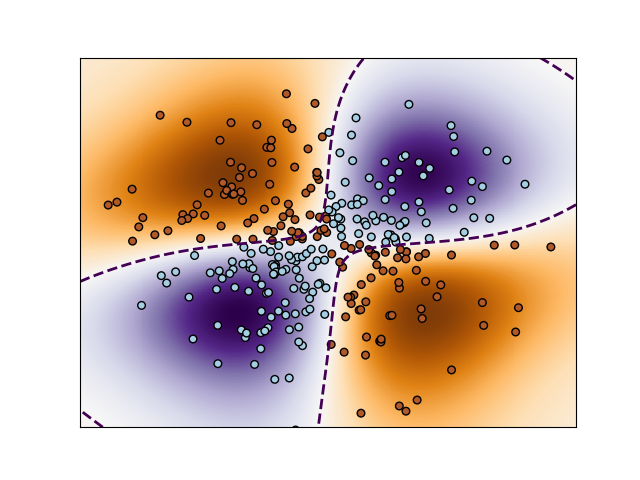
\includegraphics[width=5.4in]{../fig/nonlinearsvm.png} 
   \caption{Nonlinear separable classes in two dimensions}
   \label{fig:nonlinearsvm}
\end{figure}
\justify
Figure \ref{fig:nonlinearsvm} illustrates a nonlinear separable problem, where the two classes can not directly separated by a linear curve. This problem requires a different formulation. In this case a nonlinear function $K(X,Z)$
\begin{equation}
K: \mathbb{R}^{d}\times \mathbb{R}^{d} \rightarrow \mathbb{R}
\end{equation}
called a kernel function is required. The latter maps the data into a higher dimension space, where the data is linearly separable. Figure \ref{fig:kernelsvm} shows two classes 0 and 1 originally nonlinearly separable in two dimension.  Here it is obvious that no linear curve can be used to separate the two classes. After applying a gaussian kernel the data is map to a higher dimension where the two classes are linearly separable. This can been seen in Figure \ref{fig:kernelsvm1}, where a plan can be used to separate the two classes.
\begin{figure}[H] %  figure placement: here, top, bottom, or page
   \centering
   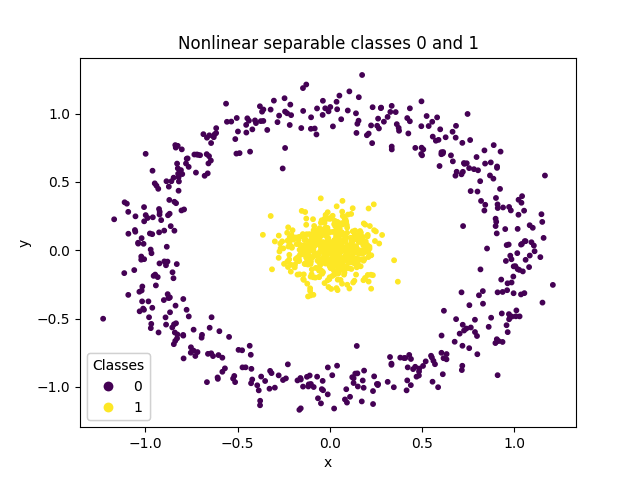
\includegraphics[width=6in]{../fig/nonlinearseparable.png} 
   %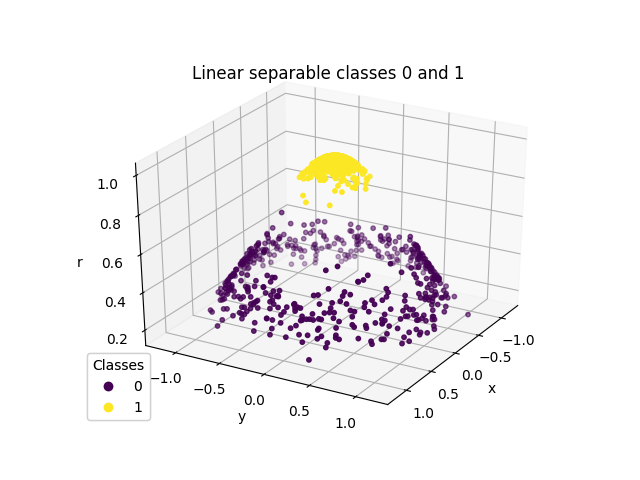
\includegraphics[width=4in]{../fig/linearseparable.png} 
   \caption{Nonlinear separable classes 0 and 1}.
   \label{fig:kernelsvm}
\end{figure}

\begin{figure}[H] %  figure placement: here, top, bottom, or page
   \centering
   %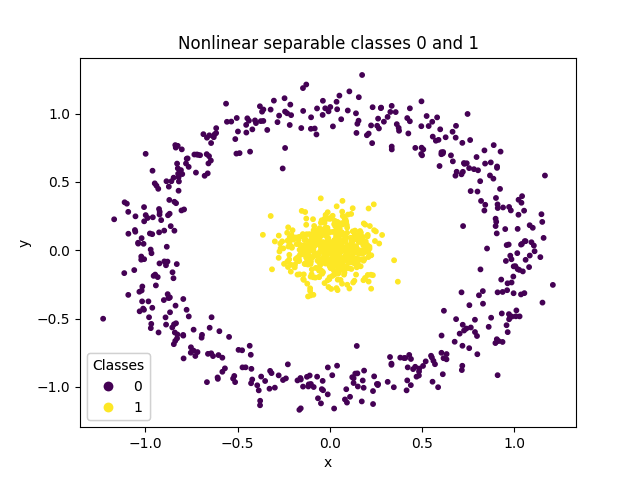
\includegraphics[width=4in]{../fig/nonlinearseparable.png} 
   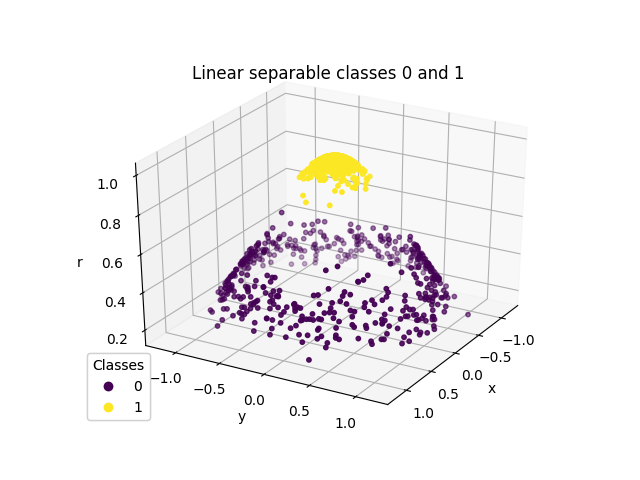
\includegraphics[width=6.5in]{../fig/linearseparable.png} 
   \caption{Linear separable classes 0 and 1 after using a gaussian kernel to map the data in higher dimension}.
   \label{fig:kernelsvm1}
\end{figure}


\justify
Example of common Kernel functions are 
\begin{itemize}
\item Linear kernel,  $K\left(X,Z\right) = X^{T}Z$
\item Polynomial of degree $q$ kernel, $K\left(X,Z\right) = \left(1+X^{T}Z\right)^{q}$ 
\item Exponential kernel,  $K(X,Z) = \exp\left(-\gamma ||X-Z||\right)$ ,$\gamma\in\mathbb{R}$
\item Gaussian kernel,  $K(X,Z) = \exp\left(-\gamma ||X-Z||^{2}\right)$ ,$\gamma\in\mathbb{R}$
\end{itemize}
The nonlinear dual formulation of the SVM can now be formulated in term of the kernel function $K$ as 
\begin{equation}
\max_{\theta}\sum_{i=1}^{n}\theta_{i} - \frac{1}{2}\sum_{i=1}^{n}\sum_{j=1}^{n}\theta_{i}\theta_{j}y_{i}y_{j}K\left(\bm{X}_{i},\bm{X}_{j}\right)
\end{equation}
subjected to 
\begin{equation}
\begin{split}
\sum_{i}^{n}\theta_{i}y_{i} = 0\\
\theta_{i} \geq 0, \quad \forall i = 1,\cdots,n.
\end{split}
\end{equation}
\justify
Some of the advantages of the SVM are high classification accuracy and robustness to outliers. That is it deals very well with aberrant data points as well as missing data points. However, for nonlinear separable problems, the computation of the kernel can incur significant overhead for large data, since the complexity is $\mathcal{O}\left(n^{2}\right)$. This can however be mitigated by performing the so call \say{kernel trick}, which reduces the complexity of the computation. Detail account of the kernel trick can be found in [reference]. 
%%%%%%%%%%%%%%%%%%%%%%%%%%%%%%%%%%%%%%%%%%%%%%%%%%%%%%%%%%%%%%%%%%%%%%%%%%%%%%%%%%%%%%%%%%%%%%%%%%%
%%%%%%%%%%%%%%%%%%%%%%%%%%%%%%%%%%%%%%%%%%%%%%%%%%%%%%%%%%%%%%%%%%%%%%%%%%%%%%%%%%%%%%%%%%%%%%%%%%%
\section{An overview of wavelet transform}
\label{sec:wavelet}
The appearance of a crack in a bearing, generates short duration periodic high frequency pulses. The Fourier transform is not well equip to detect the time of occurrence of the pulses, since it only provides frequency and amplitude information. A better approach could be the short-time Fourier transform, where the entire interval is divided into small subintervals. The Fourier transform can then be applied on each subinterval. However, this method does not accurately detect the time at which the pulses occur, since the Fourier basis function are not localized in time, \cite{albert09}. And there comes the wavelet transform in the scene.  
\begin{figure}[H] %  figure placement: here, top, bottom, or page
   \centering
   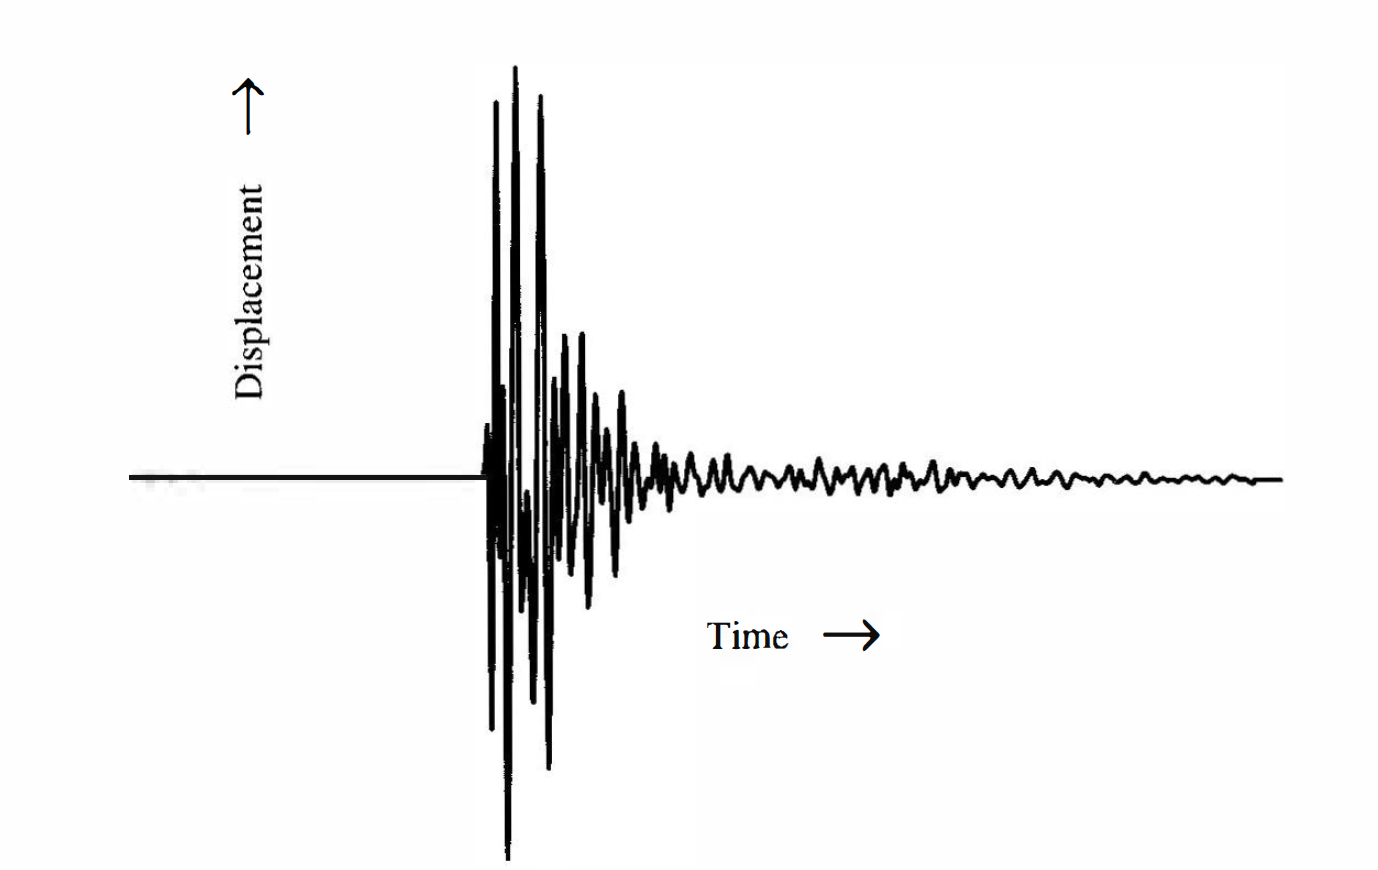
\includegraphics[width=4.5in]{../fig/seismicwave.png} 
   \caption{Example of a seismic trace. Taken from \cite{albert09}}
   \label{fig:seismicwave}
\end{figure}
\justify
Wavelet transform is a signal analysis tool that decomposes a signal into its subcomponents by using orthonormal and (sometime localized) basis functions called wavelets. The latter were originally applied in seismic survey in order to detect seismic trace \cite{albert09}. Figure \ref{fig:seismicwave} shows a seismic trace, which is a decaying high frequency short duration pulse, generated by a ground movement. Wavelets can detect and encode temporal and frequency information, unlike the Fourier transform. By construction, wavelets can \say{zoom in to observe} high frequency event and \say{zoom out} to record long and slow oscillatory movement. They can approximate non-stationary and nonlinear signal efficiently. This ability to adapt to time and space variation is due to a scaling factor build in the heart of wavelets.
\justify
Technically speaking, wavelets are family of functions generated by two functions: a scaling function denoted by $\phi$ and a wavelet function $\psi$. The former and latter are sometime refer to as \say{father wavelet} and \say{mother wavelet} respectively. By combining the scaling function and the wavelet function, one can approximate, as well as decompose a target function (signal) into its various frequency components, and record their time of occurrence. In this thesis we are interested in families of wavelets with compact support, also refer to as localized. By definition, a support of a function is a subset of the function domain, where the function does not equal to zero, but equal zero everywhere else. Being localized, these wavelets can model local short time high frequency event such as pulses emitted by a crack in a bearing. The most celebrated localized wavelet family are the Debauchies wavelets. 
\justify
The simplest wavelet belonging to the Debauchies wavelets family is the Haar wavelet, also known as Db1. The latter is the only discontinuous wavelet in that hierarchy of wavelets.
The Haar scaling function $\phi$ and the Haar wavelet function $\psi$ are given by
\begin{equation}\label{eq:haar-wavelet}
\begin{split}
\phi(x) &=
  \begin{cases}
   1 & \text{ if $0 \leq t \le 0$} \\
    0 & \text{otherwise}\\
  \end{cases}\\
  \\
\psi(t)& =
  \begin{cases}
   1 & \text{ if $0 \leq t \le \frac{1}{2}$ } \\
    -1 & \text{ if  $\frac{1}{2} \leq t \le 1$ },
    0 & \text{otherwise}
  \end{cases}
  \end{split}
\end{equation}





%%%%%%%%%%%%%%%%%%%%%%%%%%%%%%%%%%%%%%%%%%%%%%%%%%%%%%%%%%%%%%%%%%%%%%%%%%%%%%%%%%%%%%%%%%%%%%%%%%%
%%%%%%%%%%%%%%%%%%%%%%%%%%%%%%%%%%%%%%%%%%%%%%%%%%%%%%%%%%%%%%%%%%%%%%%%%%%%%%%%%%%%%%%%%%%%%%%%%%%
\section{Coupled SVM and wavelet transform for bearing anomalies detection}
\label{sec:sectionresult}


















%%%%%%%%%%%%%%%%%%%%%%%%%%%%%%%%%%%%%%%%%%%%%%%%%%%%%%%%%%%%%%%%%%%%%%%%%%%%%%%%%%%%%%%%%%%%%%%%
\blankpage
\end{document}

